\documentclass[a4paper,12pt]{report}
%general packages
\usepackage[T2A]{fontenc}
\usepackage[utf8]{inputenc}
\usepackage[english,russian]{babel}
\usepackage{circuitikz}
\usepackage{wrapfig}
\usepackage{makecell}
\usepackage{tabularx}
\usepackage{graphicx}
\usepackage{gensymb}
\usepackage{cancel} %cancel symbol
\usepackage{hyperref}
\usepackage{multirow}
\usepackage{caption}
\usepackage{subcaption}
\usepackage{amsmath}
\usepackage{changepage}
\usepackage{graphicx}
\usepackage{float}
\usepackage[english,russian]{babel}
\usepackage{amsmath, amsfonts, amssymb, amsthm, mathtools}
\usepackage{xcolor}
\usepackage{array}

%fancy header + geometry
\usepackage{fancyhdr}
\usepackage[a4paper,includehead,nomarginpar,left=15mm,right=15mm,top=15mm,headheight=10mm,bottom=20mm]{geometry}

%multi column text
\usepackage{blindtext}
\usepackage{multicol}

%parskip settings
\parindent=0ex
\setlength{\parskip}{\baselineskip}%
\setlength{\parindent}{0pt}%

%fancy notation for sets
\newcommand{\R}{{\mathbb R}}
\newcommand{\N}{{\mathbb N}}
\newcommand{\fancy}[1]{{\mathbb{#1}}}
%sgn function
\DeclareMathOperator{\sgn}{sgn}

% intersection and union symbols
\newcommand{\uni}{\cup}
\newcommand{\inter}{\cap}

\renewcommand{\footrulewidth}{0.4pt}

%\newcommand{\celsius}{$\ ^\circ C$}

%environments
\graphicspath{ {./images/} }
 
\title{Исследование применимости газа Вандер-Вальса для рассчёта эфеекта Джоуля-Томсона}
\author{Шахматов Андрей, Б02-304}
\date{\today}
  
\begin{document}
\begin{titlepage}
    \begin{center}
        {\large МОСКОВСКИЙ ФИЗИКО-ТЕХНИЧЕСКИЙ ИНСТИТУТ (НАЦИОНАЛЬНЫЙ ИССЛЕДОВАТЕЛЬСКИЙ УНИВЕРСИТЕТ)}
    \end{center}
    \begin{center}
        {\large Физтех-школа физики и исследований им. Ландау}
    \end{center}
    
    
    \vspace{3cm}
    {\huge
        \begin{center}
            \textbf{Исследование применимости газа Вандер-Вальса для рассчёта эфеекта Джоуля-Томсона}
        \end{center}
    }
    \vspace{2cm}
    \begin{flushright}
        {\LARGE Автор:\\ Шахматов Андрей Юрьевич \\
            \vspace{0.2cm}
            Б02-304}
    \end{flushright}
    \vspace{7 cm}
    \begin{center}
        Долгопрудный 2024
    \end{center}
\end{titlepage}

\pagestyle{fancy}

    \fancyhead{}
    \fancyfoot{}
    \fancyhead[L]{\rightmark}
    \fancyhead[R]{\thepage}
    \fancyfoot[R]{Работа 2.1.6 --- Эффект Джоуля---Томсона}

% \maketitle

\begin{abstract}
    Исследовано изменение температуры в опыте Джоуля-Томсона для углекислого газа. Рассчитаны 
    коэффициенты Джоуля-Томсона для углекислого газа при различных температурах в диапазоне $20 - 50$ 
    \textcelsius. Определены параметры Вандер-Вальса для углекислого газа. Проведено сравнение 
    полученных значений с табличными.      
\end{abstract}
\tableofcontents

\begin{multicols}{2}

\section{Введение}
Цель настоящей работы заключалась в определении применимости модели газа Вандер-Вальса для расчёта 
эффекта Джоуля-Томсона.  

\section{Методика}

\section{Результаты и их обсуждение}
Согласно методике определен диаметр пузырька двумя различными способами. Давление образования пузырьков 
в спирте в условных единицах шкалы монометра $P_s = &P_1&$, тогда по формуле \ref{eq:1} получим диаметр 
пузырька $d_1 = &d_exp&$ м, тогда как диаметр, измеренный под микроскопом составил $d_2 = &d&$ мм. Полученные расхождения 
можно объяснить оптическим искажением микроскопа или несовпадением диаметра иглы с диаметром пузырька.
Усреднённый результат оказался равен $d = &d_final&$ м. 
Глубины погружения отсчитанные от основания иглы оказались равны $h_1 = &h_1&$ см и $h_2 = &h_2&$ см. 
Тогда разность гидростатических давлений равна $\Delta P_1 = &dp_lin&$ Па. Тогда как непосредственное 
измерение монометром дало $\Delta P_2 = &dp_exp&$ Па. Усреднённое значение оказалось равно $\Delta P = &dp_final&$ Па. 
Полученная зависимость поверхностного натяжения от температуры представлена в таблице \ref{tab:1}. По 
полученным данным построен график зависимости \ref{fig:2}.  
\begin{figure}[H]
    \centering
    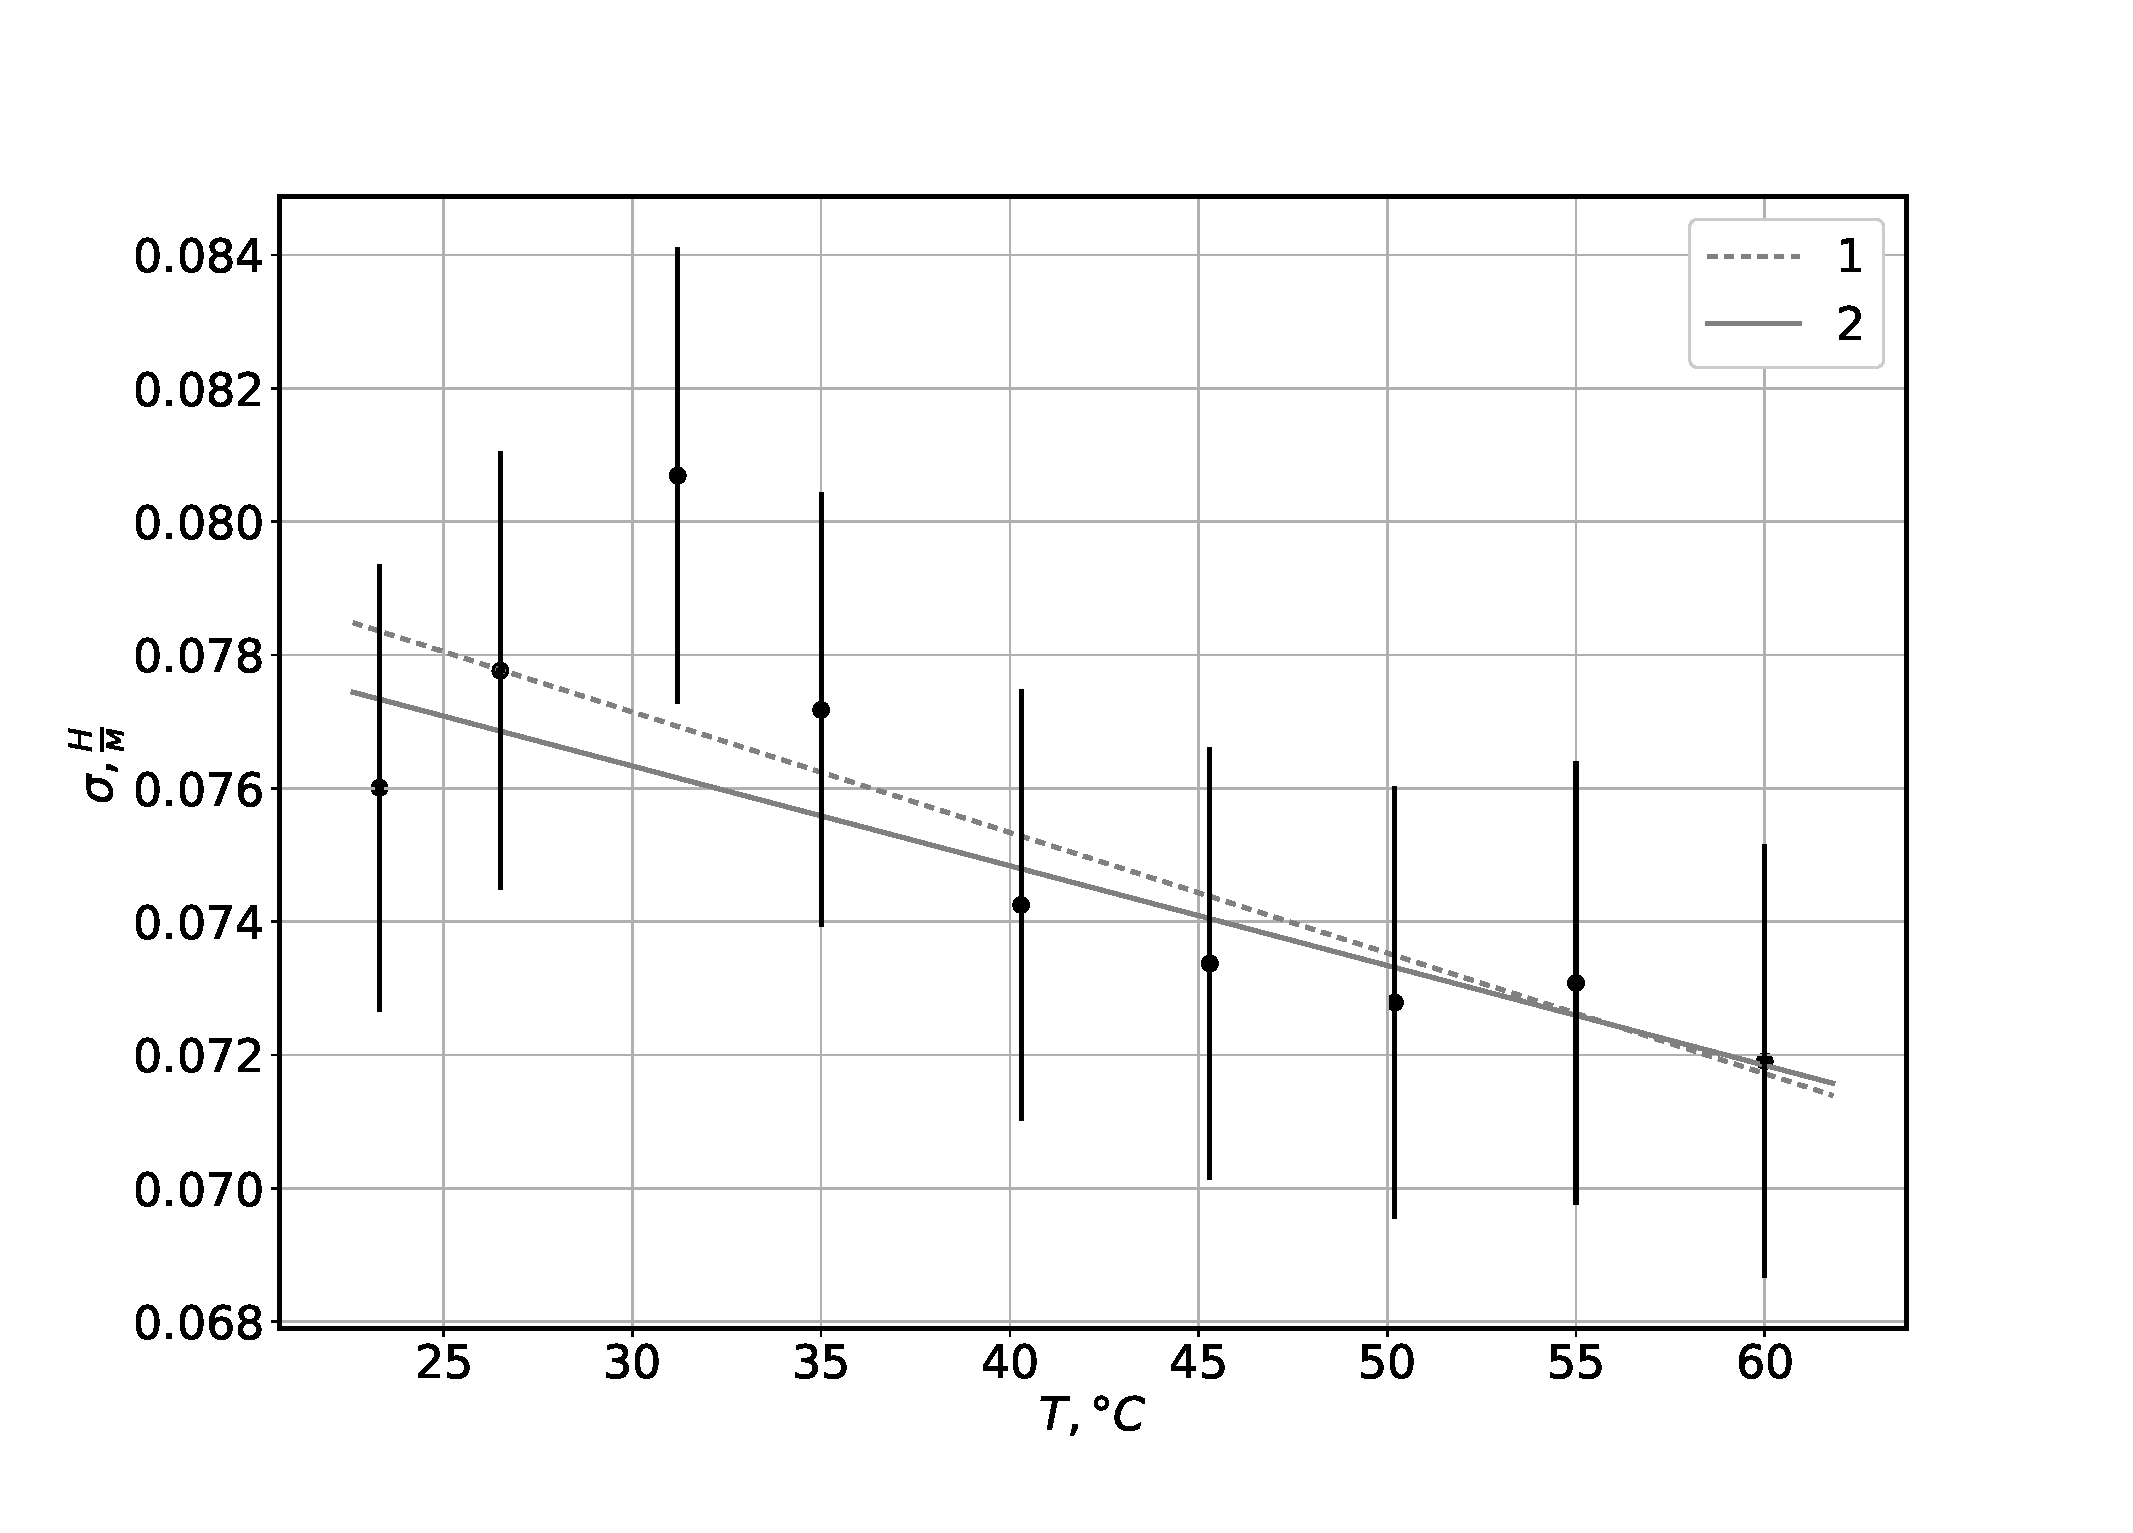
\includegraphics[width=0.7\linewidth]{sT.eps}
    \caption{График зависимости коэффициента поверхностного натяжения воды $\sigma$ от температуры $T$.
        1 - прямая, линеаризующая график зависимости с учётом всех точекя, 
        2 - прямая, линеаризующая график зависимости без учёта точек, соответствующих выбросам.}
    \label{fig:2}
\end{figure}
Из графика видно, что зависимость хорошо аппроксимируется линейной функцией при больших значениях температур, 
однако при малых температурах $(25 - 35)$ \textcelsius \, зависимость ведёт себя хаотично. Такое 
поведение возможно объяснить низкой точностью измерния монометра, а также его поломкой на заданном 
участке (нулевой уровень давления мог сбиться в процессе измерения). По этим причинам было принято решение 
исключить точку, соответствующую температуре $T = 31.2$ \textcelsius \, при дальнейших расчётах. 
Для подтверждения корректности данного решения на графике \ref{fig:2} построены две зависимости, 
линеаризирующие разные наборы данных, наглядно видно, что исключение выброшенных точек не сильно 
влияет на вид линеаризации, однако при исключении выброса полученная зависимость лучше аппроксимирует 
оставшийся набор данных.
Из линеаризации графика получено значение измерения коэффициента поверхностного натяжения от температуры 
$\frac{d\sigma }{dT} = &grad_sigma_norm&$ $\frac{\text{Н}}{\text{м}\cdot\text{К}}$. Также построены 
графики зависимости теплоты образования единицы поверхности жидкости $q = -T \frac{d \sigma}{d T}$ и 
поверхностной энергии $U$ единицы площади $F$ $\frac{U}{F} = \left( \sigma - T \frac{d \sigma }{d T} \right) $ (Рис. \ref{fig:3} и \ref{fig:4}).
\begin{figure}[H]
    \centering
    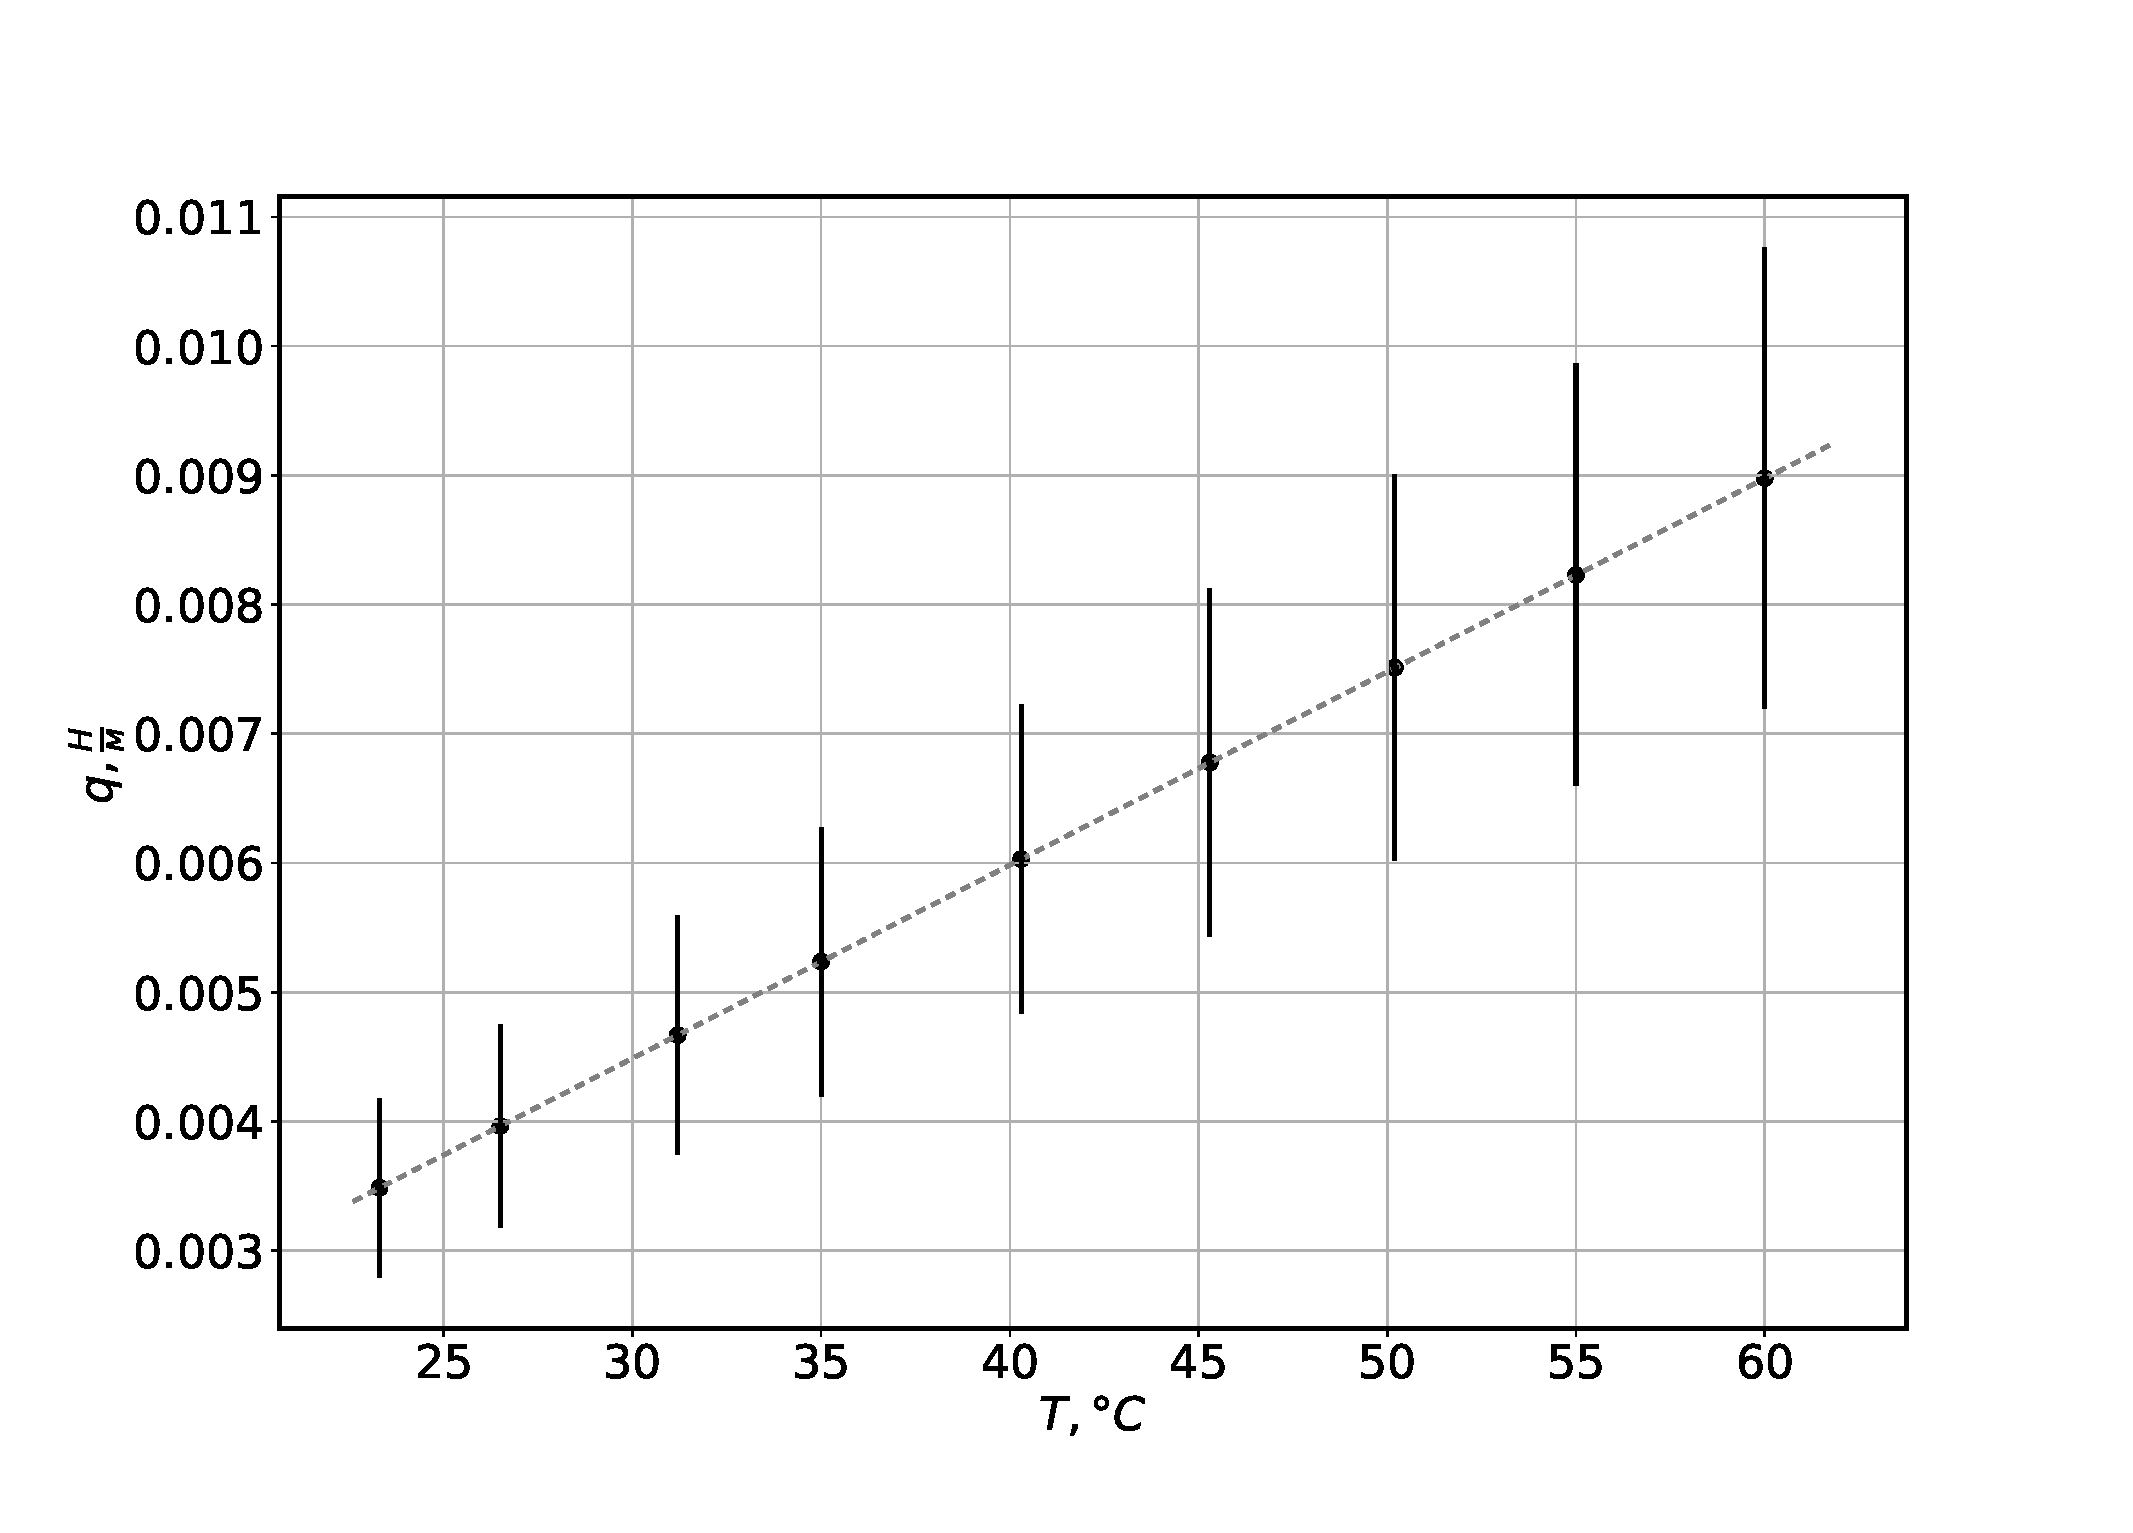
\includegraphics[width=0.7\linewidth]{qT.eps}
    \caption{График зависимости теплоты образования единицы поверхности жидкости $q$ от температуры $T$.}
    \label{fig:3}
\end{figure}
\begin{figure}[H]
    \centering
    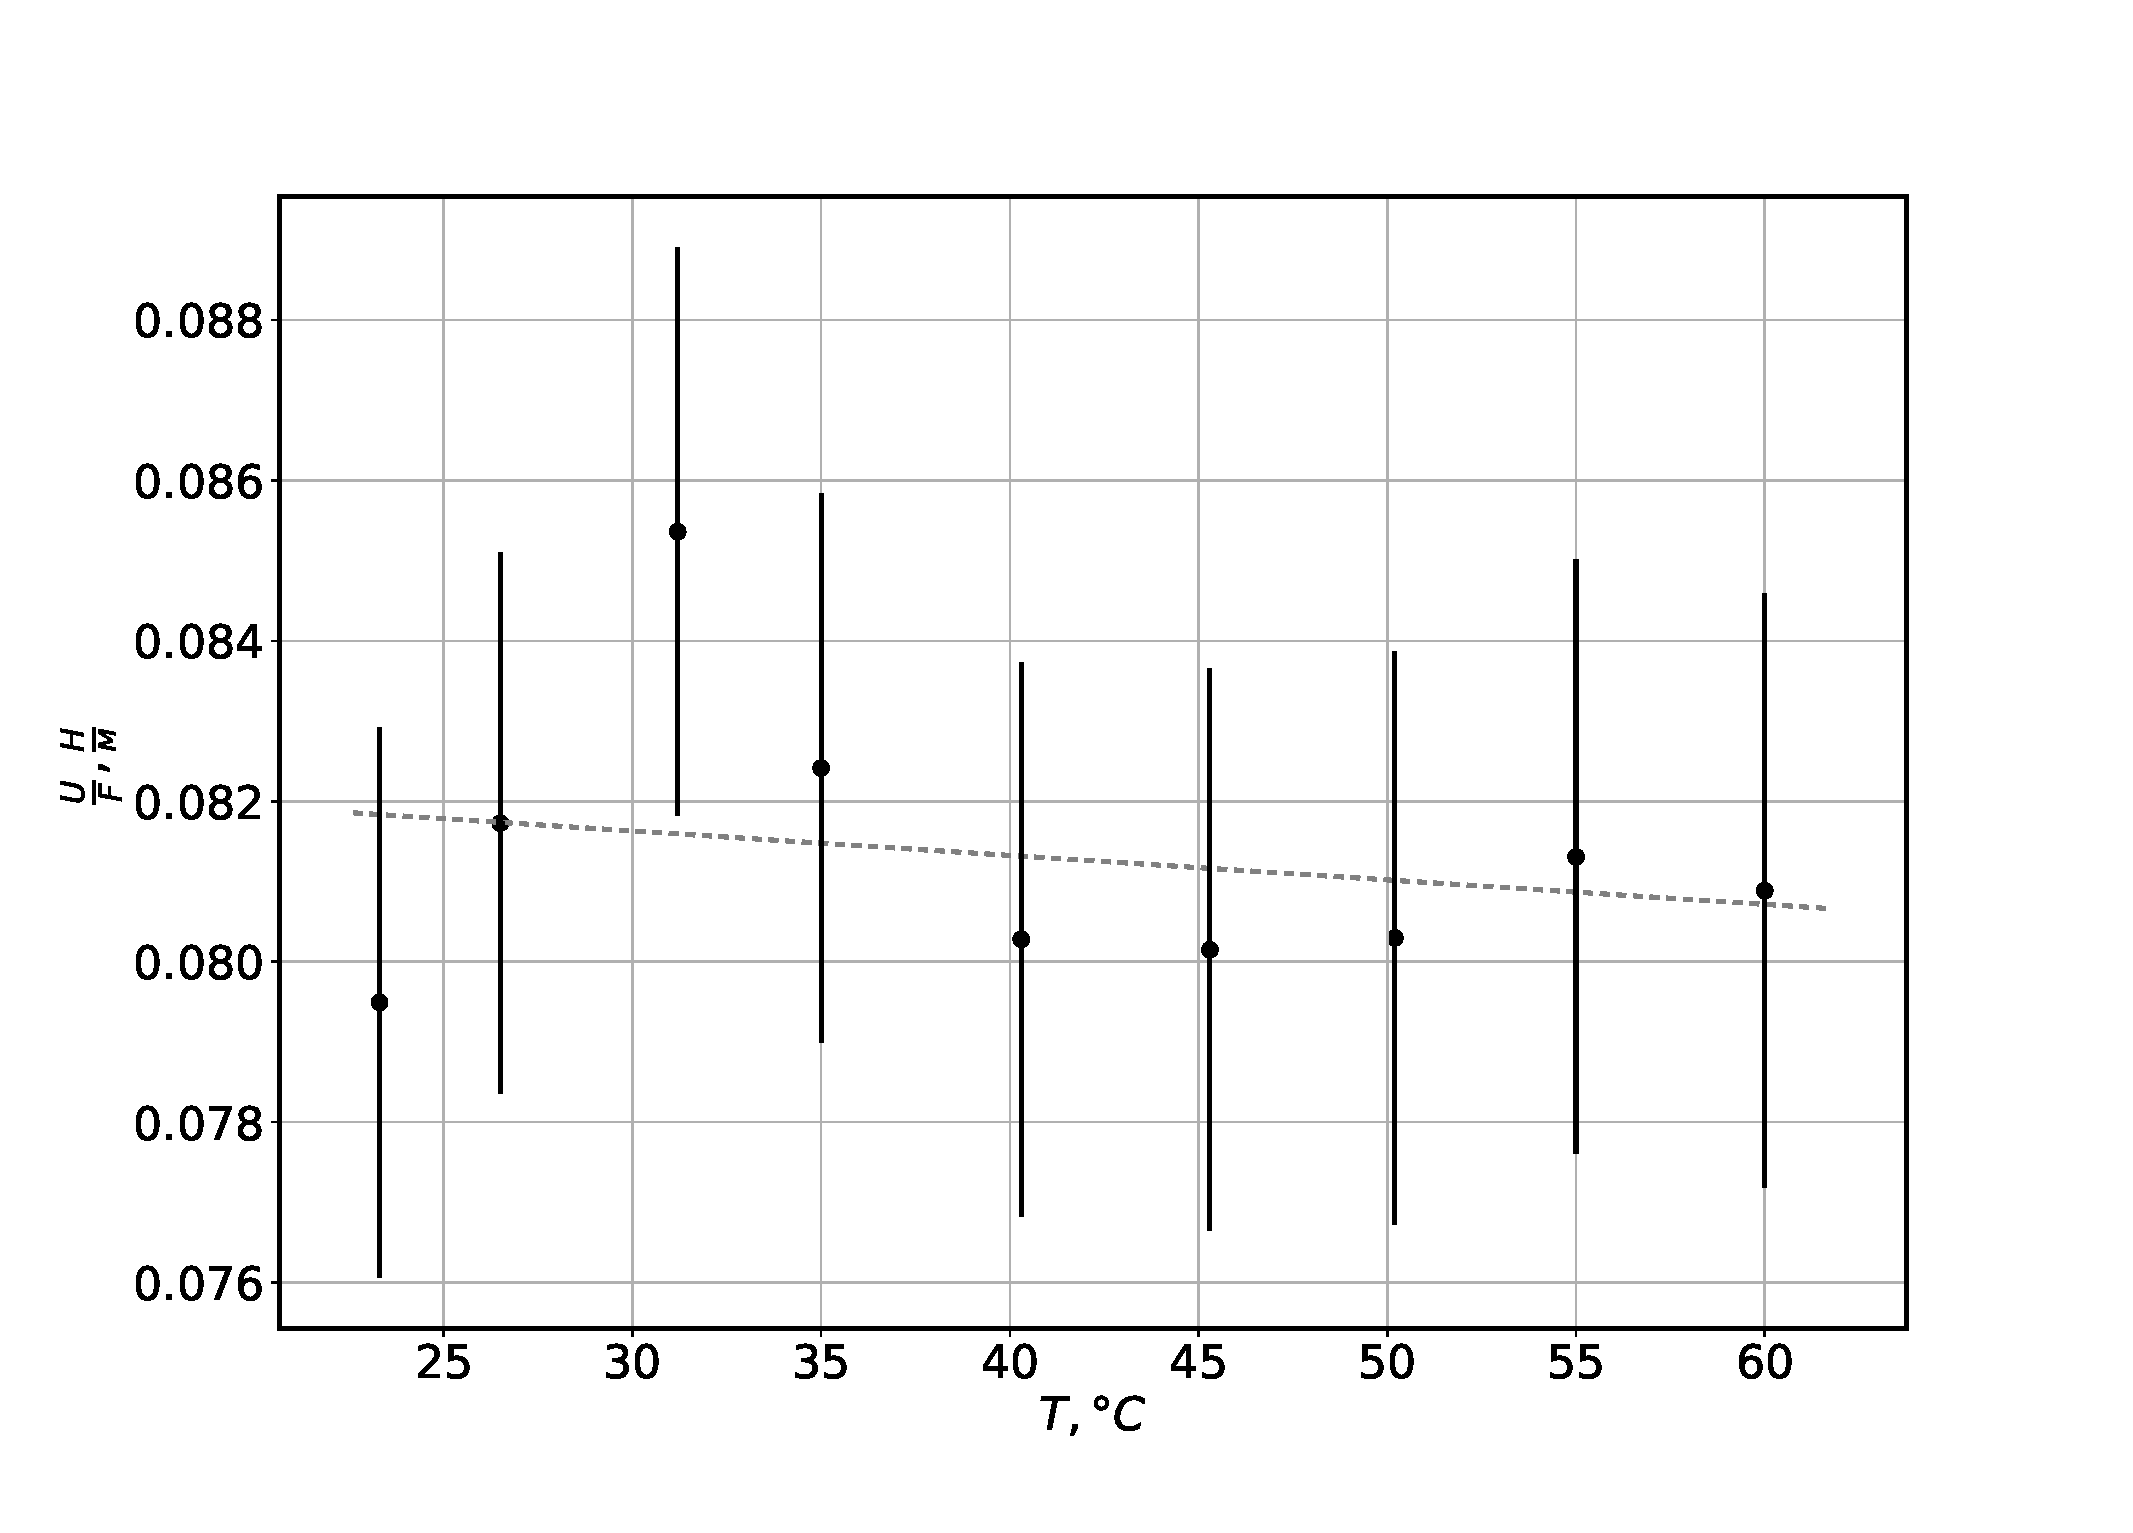
\includegraphics[width=0.7\linewidth]{qUF.eps}
    \caption{График зависимости поверхностной энергии $U$ единицы площади $F$ $\frac{U}{F}$ от температуры $T$.}
    \label{fig:4}
\end{figure}

\section{Выводы}
Измерена зависимость коэффициента поверхностного натяжения воды $\sigma$ от температуры $T$ в диапазоне 
температур (20 - 60) \textcelsius. Полученная зависимость $\sigma(T)$ хорошо аппроксимируется прямой 
с отрицательным коэффициентом наклона $\frac{d \sigma }{d T} = &grad_sigma_norm&$ $\frac{\text{Н}}{\text{м}\cdot\text{К}}$.    

\section{Использованная литература}
\begin{thebibliography}{9}
    \bibitem{LabBook}
    Лабораторный практикум по общей физике, Том 2, под редакцией А. Д. Гладуна
\end{thebibliography}

\end{multicols}

\section{Приложения}
\subsection{Параметры экспериментальной установки} \label{app_1}
При проведении эксперимента комнатная температура составила $T_0 = &T_kom&$ \textcelsius. 
Формула для перерасчёта давления из единиц шкалы монометра в реальное давление:
\[
    P = 0.2 p_m g,
\]
где $g = &g&$ $\frac{\text{м}}{\text{c}^2}$  - ускорение свободного падения. 
\subsection{Данные результатов измерений} \label{app_2}
\begin{table}[H]
    \centering
    \begin{tabular}{|l|l|l|l|l|}
        \hline
          & $T$, \textcelsius & $\sigma$, $\frac{\text{Н}}{\text{м}}$ & $\Delta T$, \textcelsius & $\Delta \sigma$, $\frac{\text{Н}}{\text{м}}$ \\
        \hline
        0 & 23.3              & 0.076                                 & 0.1                      & 0.003                                        \\
        1 & 26.5              & 0.078                                 & 0.1                      & 0.003                                        \\
        2 & 31.2              & 0.081                                 & 0.1                      & 0.003                                        \\
        3 & 35.0              & 0.077                                 & 0.1                      & 0.003                                        \\
        4 & 40.3              & 0.074                                 & 0.1                      & 0.003                                        \\
        5 & 45.3              & 0.073                                 & 0.1                      & 0.003                                        \\
        6 & 50.2              & 0.073                                 & 0.1                      & 0.003                                        \\
        7 & 55.0              & 0.073                                 & 0.1                      & 0.003                                        \\
        8 & 60.0              & 0.072                                 & 0.1                      & 0.003                                        \\
        \hline
    \end{tabular}
    \caption{Данные результатов измерений коэффициента поверхностного натяжения воды $\sigma$ от температуры $T$.}
    \label{tab:1}
\end{table}
\begin{table}[H]
    \centering
    \begin{tabular}{|l|l|l|l|l|}
        \hline
          & $T$, \textcelsius & $q$, $\frac{\text{Н}}{\text{м}}$ & $\Delta T$, \textcelsius & $\Delta q$, $\frac{\text{Н}}{\text{м}}$ \\
        \hline
        0 & 23.3              & 0.003                            & 0.1                      & 0.001                                   \\
        1 & 26.5              & 0.004                            & 0.1                      & 0.001                                   \\
        2 & 31.2              & 0.005                            & 0.1                      & 0.001                                   \\
        3 & 35.0              & 0.005                            & 0.1                      & 0.001                                   \\
        4 & 40.3              & 0.006                            & 0.1                      & 0.001                                   \\
        5 & 45.3              & 0.007                            & 0.1                      & 0.001                                   \\
        6 & 50.2              & 0.008                            & 0.1                      & 0.001                                   \\
        7 & 55.0              & 0.008                            & 0.1                      & 0.002                                   \\
        8 & 60.0              & 0.009                            & 0.1                      & 0.002                                   \\
        \hline
    \end{tabular}
    \caption{Данные зависимости теплоты образования единицы поверхности жидкости $q$ от температуры $T$.}
    \label{tab:2}
\end{table}
\begin{table}[H]
    \centering
    \begin{tabular}{|l|l|l|l|l|}
        \hline
          & $T$, \textcelsius & $\frac{U}{F}$, $\frac{\text{Н}}{\text{м}}$ & $\Delta T$, \textcelsius & $\Delta \frac{U}{F}$, $\frac{\text{Н}}{\text{м}}$ \\
        \hline
        0 & 23.3              & 0.079                                      & 0.1                      & 0.001                                    \\
        1 & 26.5              & 0.082                                      & 0.1                      & 0.001                                    \\
        2 & 31.2              & 0.085                                      & 0.1                      & 0.001                                    \\
        3 & 35.0              & 0.082                                      & 0.1                      & 0.001                                    \\
        4 & 40.3              & 0.080                                      & 0.1                      & 0.001                                    \\
        5 & 45.3              & 0.080                                      & 0.1                      & 0.001                                    \\
        6 & 50.2              & 0.080                                      & 0.1                      & 0.001                                    \\
        7 & 55.0              & 0.081                                      & 0.1                      & 0.002                                    \\
        8 & 60.0              & 0.081                                      & 0.1                      & 0.002                                    \\
        \hline
    \end{tabular}
    \caption{Данные зависимости поверхностной энергии $U$ единицы площади $F$ $\frac{U}{F}$ от температуры $T$.}
    \label{tab:3}
\end{table}
\end{document}